\chapter{Application}\label{D:application}

This chapter aims to develop the tasks introduced for the application layer in this project Gantt (see figure \ref{F:tpgp}).

\section{REST API}

As mentioned previously, it's required to develop an API ready to be used over cloud environments in order to ease creating specific and new applications over the LMS framework, and thus to demonstrate the viability of this project prototype.

Nowadays, the common and widely used format for cloud services intercommunication is JSON, as it is also used for the TCP socket API of the LMS framework. Therefore, this API middleware is going to follow such premise.

A suitable technology to work with JSON formatted messages which is widely known for its good performance is Node.js \cite{nodejs}. Node.js is an open source, cross-platform runtime environment for server-side and networking applications. It provides an event-driven architecture and a non-blocking I/O API that optimizes application's throughput and scalability. This technology is commonly used for real-time web applications. 

Moreover, working with Node.js means avoiding serialization of the JSON messages by increasing services intercommunication performance (i.e.: less computational cost and less processing time). 

Then, the common Noje.js framework for developing web applications and REST APIs is Express.js \cite{expressjs}. It's the de facto standard server framework for Node.js. So, the middleware to develop is going to use its routing system, which refers to the definition of end points (URIs with HTTP request methods like GET, POST, PUT and DELETE) to an application and how it responds to client requests.

Following is the software structure proposal for developing the HTTP RESTfull API middleware, which is responsible to translate to the TCP socket API of the LMS framework:

\begin{figure}[!htb]
\begin{center}
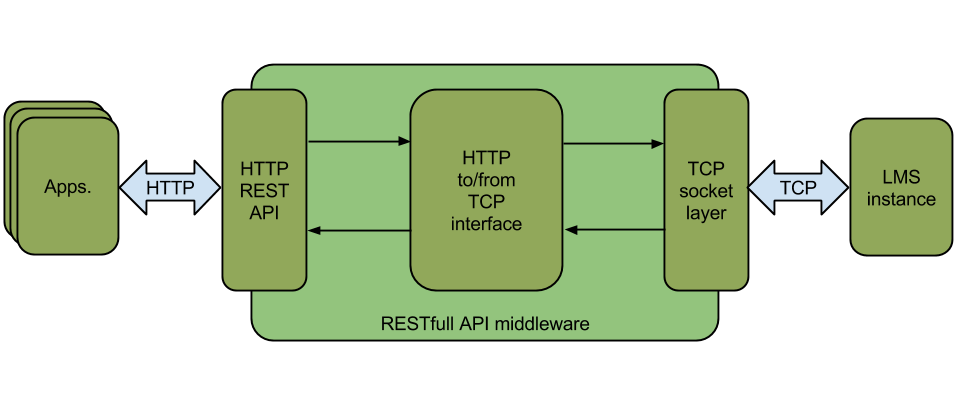
\includegraphics[width=1\textwidth]{./images/RESTAPI.png}
\caption{RESTfull API middleware architecture}
\label{F:restAPI}
\end{center}
\end{figure}

\begin{itemize}
\item HTTP REST API layer \hfill

This layer handles HTTP queries from external applications. It implements specific routes to handle specific HTTP queries. First implementation will not implement multiple LMS management but single. As shown in figure \ref{F:restAPI}.

\item Interface layer \hfill

This layer handles the body messages from the previous layer's HTTP queries and manipulates them in order to create an as much generic as possible API by adapting the messages to be sent through following layer.

\item TCP socket layer \hfill

This layer is the responsible to send and receive JSON formatted TCP socket messages between the LMS instance targeted.
\end{itemize}

As introduced in section \ref{SOA:LMS} and deeply explained in APPENDIX \ref{ANX:lmsarchfull}, there are two different management layers: the generic and the filter specific. So, by following this organization, the proposed API's structure is as shown in APPENDIX \ref{ANX:RESTAPI}.

To point out that this API is not implementing persistence because the state (managed through 'State' method) is given by the LMS instance itself. The unique sign of persistence is regarding the LMS host and port which the middleware is connected to (managed through 'Connect' and 'Disconnect' methods). Higher levels of persistence should be implemented by external applications which implies specific scenarios and requirements (i.e.: specific persistence).

Finally, in order to know how this structure and the overall middleware is implemented check APPENDIX \ref{ANX:sourceCodes} to see the code. Next chapters will demonstrate it too.

\section{Network metrics}

Network metrics could be treated as external metrics. This is because these metrics are specially dependent from sources which transmit to LMS, the receivers from LMS and the state of the network itself. Obviously, the performance of the LMS affect to the metrics gathered too, but it is intended to be minimized, at least in a gathering and presentation of the metrics' point of view.

\subsection{Input network metrics}

As said in subsection \ref{B:appLayerCH2}, input network metrics are going to be implemented by carrying out methods re-implementations given by the Live555 library, which is the library implemented for managing network streams.  

\begin{figure}[!htb]
\begin{center}
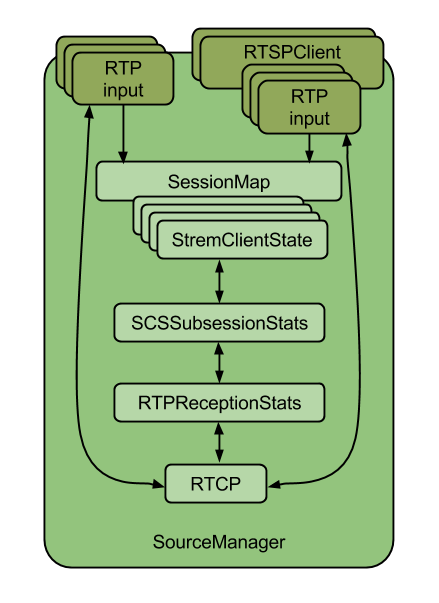
\includegraphics[width=0.45\textwidth]{./images/SourceManager.png}
\caption{Input network metrics structure}
\label{F:inms}
\end{center}
\end{figure}

By following the LiveMediaStreamer architecture structure, input network implementations are going to be implemented inside the 'liveMediaInput' structure. Concretely, a new class is implemented, called 'SCSSubsessionStats'. This class is managed by the 'StreamCleanState' class which is a class related to each stream 'Session' class managed by the 'SourceManager' class. This last class is a 'HeadFilter' class. Figure \ref{F:inms} shows the inter-class structure.

By initializing new RTP or RTSPClient sessions (i.e.: network inputs), a group of subessions is associated per each stream (i.e.: an RTP session has one subsession associated and the RTSPClient session has as many subsessions as accepted from the SDP that defines different RTP sessions).

When a new subsession is set, then, automatically, a new RTPReceiverStats class is initialized. This Live555 object implements RTCP stats measurement which are only required to be treated outside. This is done at SCSSubsessionState, which creates a new schedule to periodically measure and save current state (a default granularity of 1 second is set).

The implemented method that is called periodically is as shown in APPENDIX \ref{ANX:appALG} section \ref{inmm}.

Previous algorithm prepares the metrics that are going to be presented through the state when a new state query is received. In the code is shown how metrics from Live555 library are obtained. For a more detailed insight of the overall implementation see APPENDIX \ref{ANX:sourceCodes}. Next are listed the metrics that are presented per each new state query:

\begin{itemize}
\item Bitrate: maximum, minimum and average in kbps.
\item Packet loss percentage: maximum, minimum and average.
\item Inter-packet gap: maximum, minimum and average in milliseconds.
\item Jitter: maximum, minimum and current inter-packet gap variation in microseconds.
\end{itemize}

All these metrics are measured through previous algorithm shown which is scheduled each second (it is the default value set for all metrics gathered indeed). Concretely the bitrate is measured by knowing the overall number of octets (i.e.: bytes) received during each scheduled period and the elapsed time given by the Live555 library implementation:

\begin{equation}\label{E:bitrate}
average\ bitrate (kbps) = 8 \cdot \frac{kbytes\ receivd\ now}{elapsed\ seconds}
\end{equation}

Moreover, the maximum and the minimum are the last maximum and minimum average bitrates obtained, and this is done for all other metrics.

Then, it is important to remark that the jitter is measured as the estimate of the statistical variance of the RTP data interarrival time to be inserted in the interarrival jitter field of reception reports (in microseconds), and this is already internally done by the Live555 library. So, what is presented is the current jitter value at the beginning of each new schedule.

Another metric that might be of interest is the time delay from the stream source but it is discarded due to not being offered from Live555 library. Moreover, to be implemented at SCSSubsessionStats class level has been discarded due to is computational cost and complexity to develop such requirement. But, to point out that it is not a high priority required metric due to take into account that this issue is out of LMS performance scope and if there are network performance problems they can be detected through other metrics already gathered.


\subsection{Output network metrics}

As done in previous section, output network metrics are going to be implemented by carrying out methods re-implementations given by the Live555 library, which is the library implemented for managing network streams.

This implementation has been much more difficult to be achieved due to not having control of the RTPSink class of the Live555 library in the sense that when it is created neither deleted. Previous developments before the final version where based over the RTPSink re-implementation already done per each OnDemandServerMediaSubsession (Live555 library class), which is also re-implemented by QueueServerMediaSubsession (LMS framework class). But the implementation was still losing the specific RTPSink instance of specific subsession.

In order to go on the development an e-mail was sent to the Live555 developers mailing list, concretely to the head developer of the library, thanks to his replay the solution was clarified (see APPENDIX \ref{ANX:emailRoss}).

So, the best option, as suggested by Ross, was to re-implement the RTCPInstance class per each inheriting class of the OnDemandServerMediaSubsession class, concretely the inheriting classes of the QueueServerMediaSubsession class. 

\begin{figure}[!htb]
\begin{center}
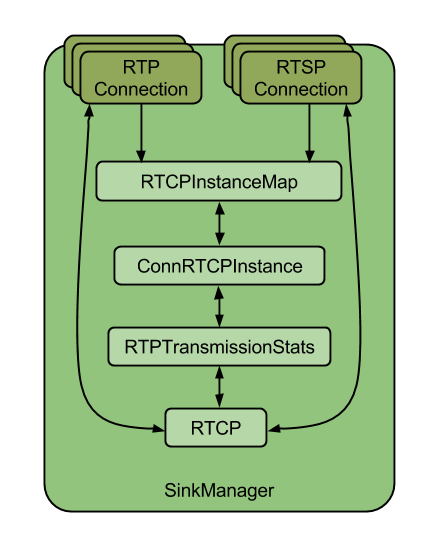
\includegraphics[width=0.45\textwidth]{./images/SinkManager.png}
\caption{Output network metrics structure}
\label{F:onms}
\end{center}
\end{figure}

In figure \ref{F:onms} is shown the relationship between the SinkManager class with both possible types of connections (i.e.: RTP or RTSP). Each Connetion object has a map of objects of the re-implemented RTCPInstance class, called ConnRTCPInstance (i.e.: RTCP instances per each connection). Then, each time a new specific RTP connection or any QueueServerMediaSubsession (RTSP connection, from RTSP server) is created, a ConnRTCPInstance is associated in order to start gathering the statistics offered from Live555 library. This is shown in APPENDIX \ref{ANX:appALG} section \ref{onmm} piece of code by showing the method which is periodically called (default periodicity value is set to 1 second), as done for the input network metrics.

In this case, the delay metric is offered from the Live555 library, which is gathered.

Finally, presented metrics are as shown next:

\begin{itemize}
\item Bitrate: maximum, minimum and average in kbps.
\item Packet loss percentage (ratio): maximum, minimum and current.
\item Round trip delay: maximum, minimum and current in milliseconds.
\item Jitter: maximum, minimum and current inter-packet gap variation in microseconds.
\end{itemize}

All these metrics are measured by applying the same patterns as done for the input network metrics.

\section{Pipeline metrics}

Following metrics are intended to be exposed as the internal metrics. It's important to point out that the measurements behind are really responsive to the overall performance of the LMS framework. Therefore, to achieve the minimum computational cost is a must. Then, as introduced in subsection \ref{B:appLayerCH2}, the optimal solutions to gather and measure such metrics is as shown next. But, first of all, let's pick up the example figure of a pipeline from APPENDIX \ref{ANX:lmsarchfull} in order to showcase the internal pipeline structure of the LMS framework. This will help understanding next two implementations.

\begin{figure}[!htb]
\begin{center}
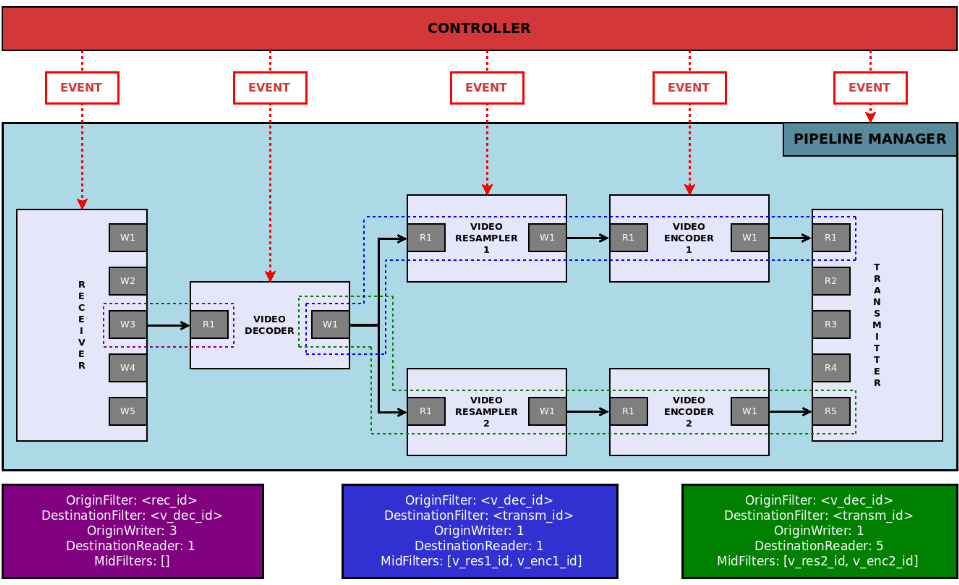
\includegraphics[width=0.9\textwidth]{./images/LMSpipelineBasicOne.png}
\caption{LMS framwork's internal pipeline structure example}
\label{F:lmsps}
\end{center}
\end{figure}

To point out that in figure \ref{F:lmsps} the arrows are the queues which interconnect each filter's writer with another filter's reader. Writers and readers are subclasses of the IOInterface class.

\subsection{Delay}

First of all, to emphasize that this metric is related to the time which data (i.e.: a video frame, an audio sample,\ldots) takes to be processed from an origin point to an end point by an unique given path, and this is measured thanks to a given and required time: the data's timestamps. Data inside the LMS source code is known as a "frame", which can be an audio frame (i.e.: sample), a H264 NAL unit, a raw frame, \ldots 

The delay time isn't considered to be measured per each filter in order to not affect the overall performance but each measured time involves an origin filter which resets the timestamps. These origins are the Head (i.e.: receiver filter) and OneToMany (i.e.: audio and video mixer filters) filters. These filters reset the frames' timestamps in order to reach and control an internal synchronization, and this is due to the fact that these filters have many outputs (i.e.: writers) or many inputs (i.e.: readers) and they require synchronizing their outputs in order to assure one point of time control inside the LMS framework, whatever the scenario configured.

So, in order to measure the delay it is important to note that a pipeline isn't composed by an unique path (see APPENDIX \ref{ANX:lmsarchfull} for clarifications) but multiple paths. This fact implies that it's not possible to measure an unique overall delay time per frame which goes over the pipeline (indeed there is a special case, and this is when there is a unique path that defines the pipeline itself, an unique path), or at least it's not suitable for performance issues, but it can be done for external applications which know the scenario configuration and gathers such metrics. Therefore, this is solved by splitting the measurements by paths. And this is an optimal measurement: the delay is given by the differential time measured by the last reader of the path (i.e.: the reader of the destination filter).

In APPENDIX \ref{ANX:appALG} section \ref{pdmm} is shown the method which implements the measurement inside the Reader class.

So, what is done is to measure the average delay of a frame by a given window time (default is configured to 1 second) with a resolution of microseconds. And this means measuring from the origin time, which, as said, is set by the origin filters (i.e.: the beginning of a path, starting from a writer), to each reader of the path (i.e.: each filter). But, the delay time presented is from the beginning (i.e.: initial writer of the path) until the last reader. See figure \ref{F:lmsps} where different path examples are illustrated.

\subsection{Losses}

This metric is following a similar criteria as the previous one. This is solved by measuring at the same point, but it's done when flushing frames at the reader side (as introduced in section \ref{B:appLayerCH2}). In order to reach minimal computational cost, the measurement is just a counter of the overall data losses when calling the flush methods. What is done is a method encapsulation by defining a parent method that is just incrementing its reader counter and then it calls the specific flush implementation per each data/frame type.

Then, in order to properly present it to external applications it is required to be presented at a path level as done for the delay metrics. So, in this case it is only required to sum up the overall losses of the path's readers.

It is important to note that this metric is not referenced to a total data processed or at any time point, but specific problem detections are achieved thanks to measuring its continuity. This means that if this value is incrementing gradually then the system is not working properly. Such detections might imply fast increments on its continuity (differential increase). 


Finally, as a section corollary, Pipeline metrics are measured when flushing frames (discarding) or when a reader is able to remove a frame from its belonging queue. 
